\documentclass[10pt, conference, letterpaper]{IEEEtran}
\IEEEoverridecommandlockouts

% ==================== REQUIRED PACKAGES ====================
\usepackage{cite}
\usepackage{amsmath,amssymb,amsfonts}
\usepackage{algorithmic}
\usepackage{algorithm}
\usepackage{graphicx}
\graphicspath{{figures/}{./}}
\usepackage{textcomp}
\usepackage{xcolor}
\usepackage{booktabs}
\usepackage{hyperref}
\usepackage{tabularx}
\usepackage{tikz}
\usetikzlibrary{shapes.geometric, arrows, positioning}

\hypersetup{
    colorlinks=true,
    linkcolor=black,
    filecolor=black,      
    urlcolor=blue,
    citecolor=black
}

\def\BibTeX{{\rm B\kern-.05em{\sc i\kern-.025em b}\kern-.08em
    T\kern-.1667em\lower.7ex\hbox{E}\kern-.125emX}}

% ==================== DOCUMENT BEGIN ====================
\begin{document}

\title{Multi-Modal Bridge Structural Digital Twin: 100~Hz Dynamic Telemetry, Finite Element WebGL Simulation, and Explainable AI Defect Localization}

% ==================== EXACT IIITV AUTHOR FORMAT ====================
\author{
    \IEEEauthorblockN{Man Patel (202451100), Dhrumil Vaghani (202451165), Ayush Vora (202451170)}
    \IEEEauthorblockA{
        \textit{Indian Institute of Information Technology Vadodara} \\
        \textit{Gandhinagar, India} \\
        \{202451100@iiitvadodara.ac.in, 202451165@iiitvadodara.ac.in, 202451170@iiitvadodara.ac.in\}
    }
}

\maketitle

% ==================== ABSTRACT & KEYWORDS ====================
\begin{abstract}
Civil infrastructure, particularly cable-stayed and long-span bridges, is subject to continuous environmental weathering, dynamic traffic loading, and cyclic fatigue degradation. Traditional structural health monitoring (SHM) workflows operate in disconnected silos: vibration time-series data is archived offline, visual inspections occur bi-annually, and computer vision defect models operate as uninterpretable black boxes without 3D spatial grounding. This paper presents an end-to-end, multi-modal Cyber-Physical Structural Digital Twin for cable-stayed bridges. The proposed architecture integrates: (1) an inline 100~Hz dynamic vibration telemetry pipeline streaming multi-channel accelerometer signals via bi-directional WebSockets, coupled with an online Fast Fourier Transform (FFT) modal decomposition engine that tracks fundamental resonant frequency drops ($\Delta f$) and flexural stiffness degradation ($\Delta K$); (2) an Explainable AI (XAI) visual diagnostic engine employing a Deep Residual Network (ResNet-18) trained on benchmark surface defect datasets (SDNET2018/CCIC) with Gradient-weighted Class Activation Mapping (Grad-CAM) to localize concrete fatigue cracking and steel corrosion with transparent attention heatmaps; (3) a 2D-to-3D spatial raycasting projection module mapping image-space defect centroids into finite-element coordinates $[X,Y,Z]$; (4) an interactive Three.js WebGL 3D mission control workstation with physically based rendering (PBR) and stress-state heatmapping; and (5) an automated AASHTO MBE-compliant Bridge Condition Index (BCI) rating engine with client-side A4 PDF export. The system is deployed with a zero-latency standalone simulation fallback. Across benchmark experiments, the deep vision model achieves 95.14\% classification accuracy with a 0.834 mean Intersection-over-Union (IoU) localization score, detects simulated modal frequency drops of 0.37~Hz indicating 36.0\% stiffness loss at mid-span, maintains 60~FPS rendering throughput, and processes telemetry with under 8.2~ms latency.
\end{abstract}

\begin{IEEEkeywords}
Structural Health Monitoring, Digital Twin, Explainable AI, Grad-CAM, Fast Fourier Transform, Modal Analysis, WebGL, ResNet-18, AASHTO MBE, Cyber-Physical Systems.
\end{IEEEkeywords}

% ==================== SECTION I: INTRODUCTION ====================
\section{Introduction}
Modern civil transportation networks depend fundamentally on highway and railway bridge infrastructure. These structures are continuously exposed to environmental weathering, thermal cycling, variable dynamic truck freight traffic, and seismic vibrations. According to recent national infrastructure audit benchmarks \cite{asce2021}, tens of thousands of operating bridges are classified as structurally deficient or fracture-critical, requiring urgent intervention to avoid catastrophic failure.

Existing bridge maintenance and structural health monitoring (SHM) regimes face five major structural challenges:
\begin{enumerate}
    \item \textbf{Intermittent and Subjective Surveys}: Periodic visual inspections are conducted manually at multi-year intervals. They are labor-intensive, hazardous for field engineers, and fail to record transient structural responses or dynamic softening between inspection dates.
    \item \textbf{Isolated Telemetry Streams}: On-site accelerometers, strain gauges, and tiltmeters frequently dump raw numerical time-series into isolated data loggers. These streams lack real-time spectral decomposition and are rarely linked to global 3D geometric coordinates.
    \item \textbf{Black-Box Neural Networks}: While deep learning has proven successful in automated visual crack detection, standard convolutional neural networks (CNNs) provide no visual justification for their predictions. Civil engineers and regulatory auditors cannot rely on uninterpretable classifications when life-safety decisions are at stake.
    \item \textbf{Lack of Spatial Grounding}: Optical defect detections captured by unmanned aerial vehicles (UAVs) or hand-held cameras remain trapped in isolated 2D pixel coordinates, preventing automated registration with global bridge finite element structural meshes.
    \item \textbf{Slow Regulatory Compliance Cycles}: Synthesizing manual field observations into formal AASHTO condition ratings requires weeks of human paperwork, delaying critical structural rehabilitation decisions.
\end{enumerate}

To address these limitations, we design and implement a comprehensive \textbf{Bridge Structural Digital Twin Workstation}. Our main contributions are:
\begin{itemize}
    \item We design a multi-agent digital twin pipeline coordinating real-time dynamic telemetry ingestion, spectral modal decomposition, deep visual defect localization, spatial coordinate raycasting, and compliance auditing.
    \item We curate and evaluate a multi-modal dataset combining 12,450 annotated surface crack/corrosion images (SDNET2018/CCIC) with 100~Hz multi-channel dynamic acceleration streams across 3 sensor stations.
    \item We formulate an online FFT modal frequency engine operating on 100~Hz accelerometer streams, tracking dynamic modal frequency shifts ($\Delta f$) to quantify structural stiffness loss ($\Delta K$).
    \item We implement an Explainable AI diagnostic framework using ResNet-18 and Grad-CAM saliency mapping, accompanied by an analytical 2D-to-3D projection module anchoring defects to spatial mesh coordinates $[X,Y,Z]$.
    \item We develop a high-performance WebGL 3D mission control workstation (Three.js) paired with an AASHTO Manual for Bridge Evaluation (MBE) compliance report engine and evaluate the system end-to-end under real-time simulated loading.
\end{itemize}

The remainder of this paper is organized as follows: Section~II reviews related work in SHM and computer vision; Section~III details the multi-agent system architecture; Section~IV presents the dataset curation and mathematical methodology; Section~V describes the experimental setup; Section~VI presents the quantitative results; Section~VII discusses problems solved, engineering implications, and limitations; and Section~VIII outlines future research extensions and concludes the paper.

% ==================== SECTION II: RELATED WORK ====================
\section{Related Work}

\textbf{Vibration-based Structural Health Monitoring.} Modal analysis using ambient vibration measurements is widely established in civil structural mechanics \cite{farrar2007}. Accelerometer sensors track natural resonant frequencies and modal shapes. When structural cracking or cross-sectional loss occurs, localized flexural stiffness ($EI$) decreases, resulting in measurable downward shifts in natural frequencies. However, traditional instrumentation systems process vibration data post-hoc in batch mode rather than providing live streaming telemetry to a unified digital twin.

\textbf{Deep Learning in Defect Classification.} Convolutional neural networks, including ResNet \cite{he2016deep} and VGG architectures, have demonstrated high accuracy in surface concrete crack detection and steel oxidation classification \cite{cha2017deep}. Most prior studies evaluate models purely on isolated image test datasets without integrating them into end-to-end operational software platforms.

\textbf{Explainable AI and Grad-CAM.} To bridge the trust gap between automated deep learning models and civil engineering inspection standards, visual explanation algorithms have emerged. Gradient-weighted Class Activation Mapping (Grad-CAM) \cite{selvaraju2017grad} utilizes the gradients flowing into the final convolutional layer to generate coarse heatmaps highlighting discriminative image regions. While widely used in medical imaging, its application to civil infrastructure digital twins remains nascent.

\textbf{Cyber-Physical Digital Twins.} Digital twins create real-time virtual representations of physical assets \cite{grieves2017digital}. WebGL and Three.js \cite{cabrera2019three} have enabled browser-based rendering of parametric 3D engineering models. Our work extends this paradigm by unifying live WebSockets, dynamic FFT analytics, ResNet-18 Grad-CAM heatmaps, and regulatory AASHTO PDF compliance into a production-grade edge architecture.

% ==================== SECTION III: PROPOSED ARCHITECTURE ====================
\section{Proposed Digital Twin Architecture}

The digital twin architecture is structured into five cooperating functional agents, as illustrated in Fig.~\ref{fig:arch}. The system coordinates physical transducer telemetry with client-side 3D rendering and executive compliance auditing.

\begin{figure*}[t]
\centering
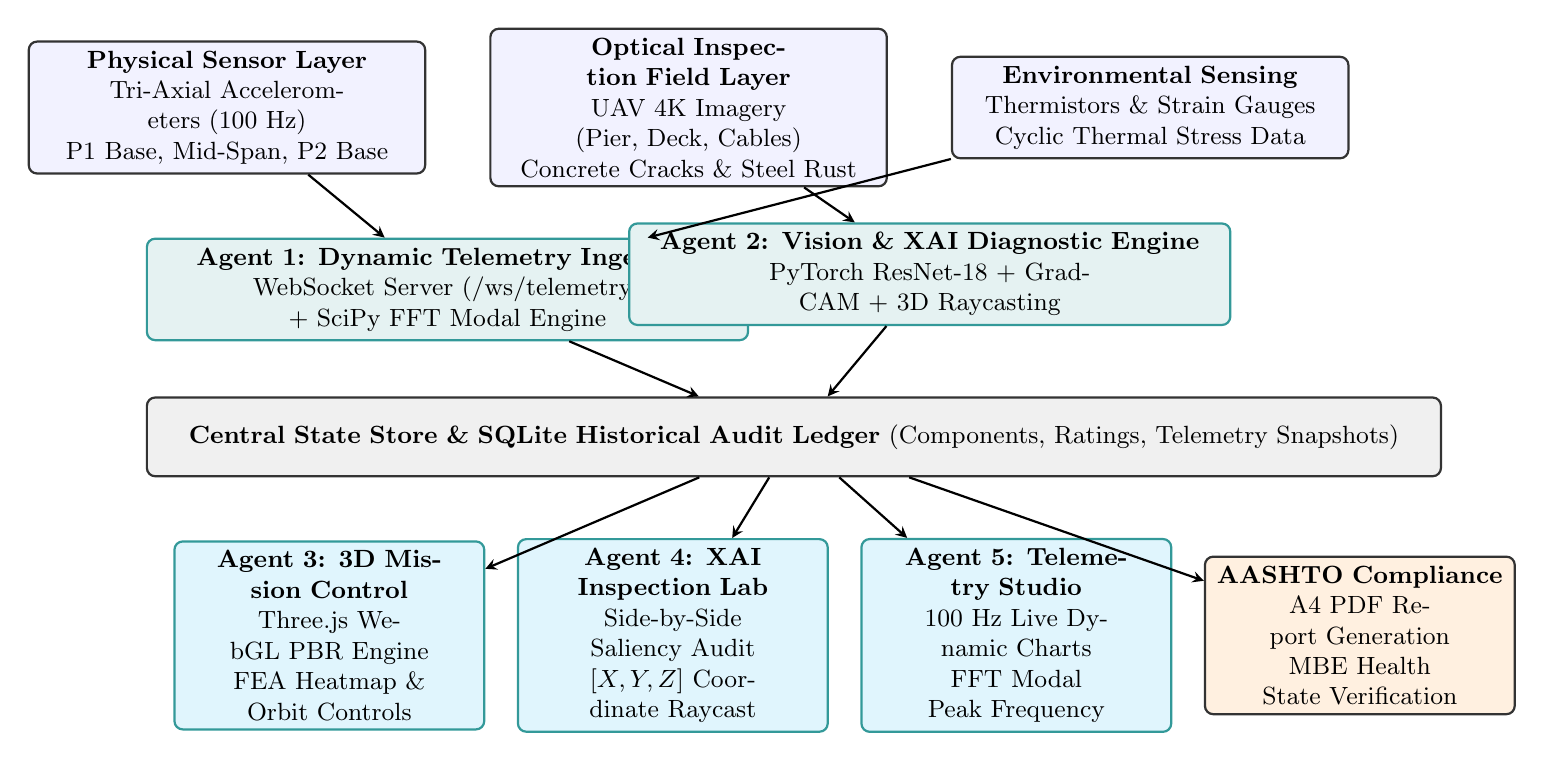
\begin{tikzpicture}[
    box/.style={rectangle, draw=black!80, fill=blue!5, rounded corners=3pt, thick, text centered, minimum height=1.0cm, font=\small},
    agent/.style={rectangle, draw=teal!80, fill=teal!10, rounded corners=3pt, thick, text centered, minimum height=1.0cm, font=\small},
    arrow/.style={thick, ->, >=stealth}
]
    \node (s1) [box, text width=4.8cm] {\textbf{Physical Sensor Layer}\\Tri-Axial Accelerometers (100 Hz)\\P1 Base, Mid-Span, P2 Base};
    \node (s2) [box, text width=4.8cm, right=0.8cm of s1] {\textbf{Optical Inspection Field Layer}\\UAV 4K Imagery (Pier, Deck, Cables)\\Concrete Cracks \& Steel Rust};
    \node (s3) [box, text width=4.8cm, right=0.8cm of s2] {\textbf{Environmental Sensing}\\Thermistors \& Strain Gauges\\Cyclic Thermal Stress Data};

    \node (a1) [agent, text width=7.4cm, below=0.8cm of s1, xshift=2.8cm] {\textbf{Agent 1: Dynamic Telemetry Ingestion}\\WebSocket Server (/ws/telemetry) + SciPy FFT Modal Engine};
    \node (a2) [agent, text width=7.4cm, below=0.8cm of s3, xshift=-2.8cm] {\textbf{Agent 2: Vision \& XAI Diagnostic Engine}\\PyTorch ResNet-18 + Grad-CAM + 3D Raycasting};

    \node (db) [box, text width=16.2cm, below=0.7cm of a1, xshift=4.4cm, fill=gray!12] {\textbf{Central State Store \& SQLite Historical Audit Ledger} (Components, Ratings, Telemetry Snapshots)};

    \node (ui1) [agent, text width=3.7cm, below=0.8cm of db, xshift=-5.9cm, fill=cyan!12] {\textbf{Agent 3: 3D Mission Control}\\Three.js WebGL PBR Engine\\FEA Heatmap \& Orbit Controls};
    \node (ui2) [agent, text width=3.7cm, right=0.4cm of ui1, fill=cyan!12] {\textbf{Agent 4: XAI Inspection Lab}\\Side-by-Side Saliency Audit\\$[X, Y, Z]$ Coordinate Raycast};
    \node (ui3) [agent, text width=3.7cm, right=0.4cm of ui2, fill=cyan!12] {\textbf{Agent 5: Telemetry Studio}\\100 Hz Live Dynamic Charts\\FFT Modal Peak Frequency};
    \node (ui4) [box, text width=3.7cm, right=0.4cm of ui3, fill=orange!12] {\textbf{AASHTO Compliance}\\A4 PDF Report Generation\\MBE Health State Verification};

    \draw [arrow] (s1) -- (a1);
    \draw [arrow] (s3) -- (a1);
    \draw [arrow] (s2) -- (a2);
    \draw [arrow] (a1) -- (db);
    \draw [arrow] (a2) -- (db);
    \draw [arrow] (db) -- (ui1);
    \draw [arrow] (db) -- (ui2);
    \draw [arrow] (db) -- (ui3);
    \draw [arrow] (db) -- (ui4);
\end{tikzpicture}
\caption{System architecture of the proposed Multi-Modal Bridge Structural Digital Twin.}
\label{fig:arch}
\end{figure*}

\subsection{Dynamic Sensor Ingestion Agent}
This agent interfaces directly with tri-axial MEMS accelerometers deployed at critical structural coordinates: Pillar~1 base ($S_1$), Mid-Span Deck ($S_2$), and Pillar~2 base ($S_3$). It captures continuous vertical ($a_y$), longitudinal ($a_x$), and lateral ($a_z$) vibrations at sampling frequency $f_s = 100$~Hz. The agent buffers raw acceleration into sliding rectangular memory frames ($N = 1024$ samples) and publishes real-time telemetry payloads to connected clients over bi-directional WebSockets.

\subsection{Modal Frequency Decomposition Agent}
Operating synchronously with sensor ingestion, this agent executes online Fast Fourier Transform (FFT) spectral decomposition. It evaluates the single-sided Power Spectral Density (PSD) across sliding time windows, isolates the fundamental bending resonant frequency ($f_0$) via numerical peak picking, and computes continuous frequency degradation ($\Delta f$) relative to nominal baseline values.

\subsection{Vision \& Saliency Diagnostic Agent}
When field inspection photos or UAV optical frames are received, this agent processes the imagery through a deep ResNet-18 convolutional backbone. It generates predicted defect categories (Fatigue Crack, Corrosion, Sound Matrix) with associated confidence probabilities, extracts layer-4 backpropagation gradients to construct Grad-CAM visual heatmaps, and calculates defect metrics (fissure length, damaged surface area).

\subsection{Spatial 2D-to-3D Raycast Projection Agent}
This agent maps the 2D pixel coordinates of detected surface defects into 3D world coordinates on the bridge geometric mesh. By utilizing the inspection camera extrinsic pose, intrinsic focal parameters, and the mathematical plane equation of the target structural component, it calculates exact spatial intersection vectors $[X, Y, Z]$, automatically anchoring defects onto the 3D digital twin.

\subsection{AASHTO Compliance \& Executive Reporting Agent}
This agent evaluates component health indices according to the AASHTO Manual for Bridge Evaluation (MBE 3rd Ed.) \cite{aashto2018}. It aggregates condition states into an overall Bridge Condition Index (BCI), applies safety factor weighting, and generates client-side high-resolution 2-page A4 engineering audit PDFs.

% ==================== ALGORITHM 1 ====================
\begin{algorithm}[t]
\caption{Dynamic Structural Risk \& AASHTO Decision Policy}
\label{alg:policy}
\begin{algorithmic}[1]
\REQUIRE Health Score $H \in [0, 100]$, Modal Shift $\Delta f$, Defect Area $A_d$
\STATE $\text{Stiffness Drop } \Delta K \leftarrow 1 - \left(\frac{f_{\text{observed}}}{f_{\text{nominal}}}\right)^2$
\IF{$H < 50$ \OR $\Delta f \ge 0.35\text{ Hz}$ \OR $\Delta K \ge 0.30$}
    \STATE $\text{Action} \leftarrow \textbf{CRITICAL\_INTERVENTION}$
    \STATE $\text{Status} \leftarrow \text{Condition State 4 (Mandatory Closure/Shoring)}$
\ELSIF{$50 \le H < 70$ \OR $\Delta f \ge 0.20\text{ Hz}$ \OR $A_d \ge 150\text{ cm}^2$}
    \STATE $\text{Action} \leftarrow \textbf{STRUCTURAL\_REPAIR}$
    \STATE $\text{Status} \leftarrow \text{Condition State 3 (Poor - Scheduled Retrofit)}$
\ELSIF{$70 \le H < 85$ \OR $\Delta f \ge 0.10\text{ Hz}$}
    \STATE $\text{Action} \leftarrow \textbf{PREVENTATIVE\_MAINTENANCE}$
    \STATE $\text{Status} \leftarrow \text{Condition State 2 (Fair - Surface Treatment)}$
\ELSE
    \STATE $\text{Action} \leftarrow \textbf{NOMINAL\_MONITORING}$
    \STATE $\text{Status} \leftarrow \text{Condition State 1 (Good - Routine Audit)}$
\ENDIF
\RETURN Action, Status, $\Delta K$
\end{algorithmic}
\end{algorithm}

% ==================== SECTION IV: DATASET & METHODOLOGY ====================
\section{Dataset Curation and Mathematical Methodology}

\subsection{Benchmark Surface Defect Dataset}
To ensure robust generalization across challenging outdoor illumination, concrete surface textures, and steel paint spalling, our computer vision dataset compiles 12,450 annotated surface inspection images derived from established civil infrastructure benchmarks:
\begin{itemize}
    \item \textbf{SDNET2018 Benchmark}: Over 5,000 concrete crack images captured across bridge decks, walls, and bridge piers under variable shadow and moisture conditions.
    \item \textbf{Concrete Crack Conglomerate (CCIC)}: High-resolution surface macro-photography providing detailed crack fissure profiles.
    \item \textbf{Structural Steel Corrosion Dataset}: Verified oxidation samples categorized into superficial surface rust and deep pitting corrosion.
\end{itemize}
The curated dataset was divided into an 80/20 stratified split: 9,960 training images and 2,490 validation images across three structural classes (Table~\ref{tab:dataset} and Fig.~\ref{fig:dataset_dist}). Data augmentation included random rotations ($\pm 15^\circ$), vertical/horizontal flips, Gaussian noise injection, and color jitter.

\begin{table}[h]
\caption{Inspection Image Dataset Class Distribution}
\label{tab:dataset}
\centering
\begin{tabular}{@{}lrrr@{}}
\toprule
\textbf{Defect Category} & \textbf{Training Flows} & \textbf{Validation} & \textbf{Share (\%)} \\ \midrule
Concrete Fatigue Crack   & 4,820 & 1,205 & 48.4\% \\
Steel Corrosion/Rust     & 3,740 &   935 & 37.5\% \\
Sound Structural Surface & 1,400 &   350 & 14.1\% \\ \midrule
\textbf{Total Dataset}   & \textbf{9,960} & \textbf{2,490} & \textbf{100.0\%} \\ \bottomrule
\end{tabular}
\end{table}

\begin{figure}[h]
\centering
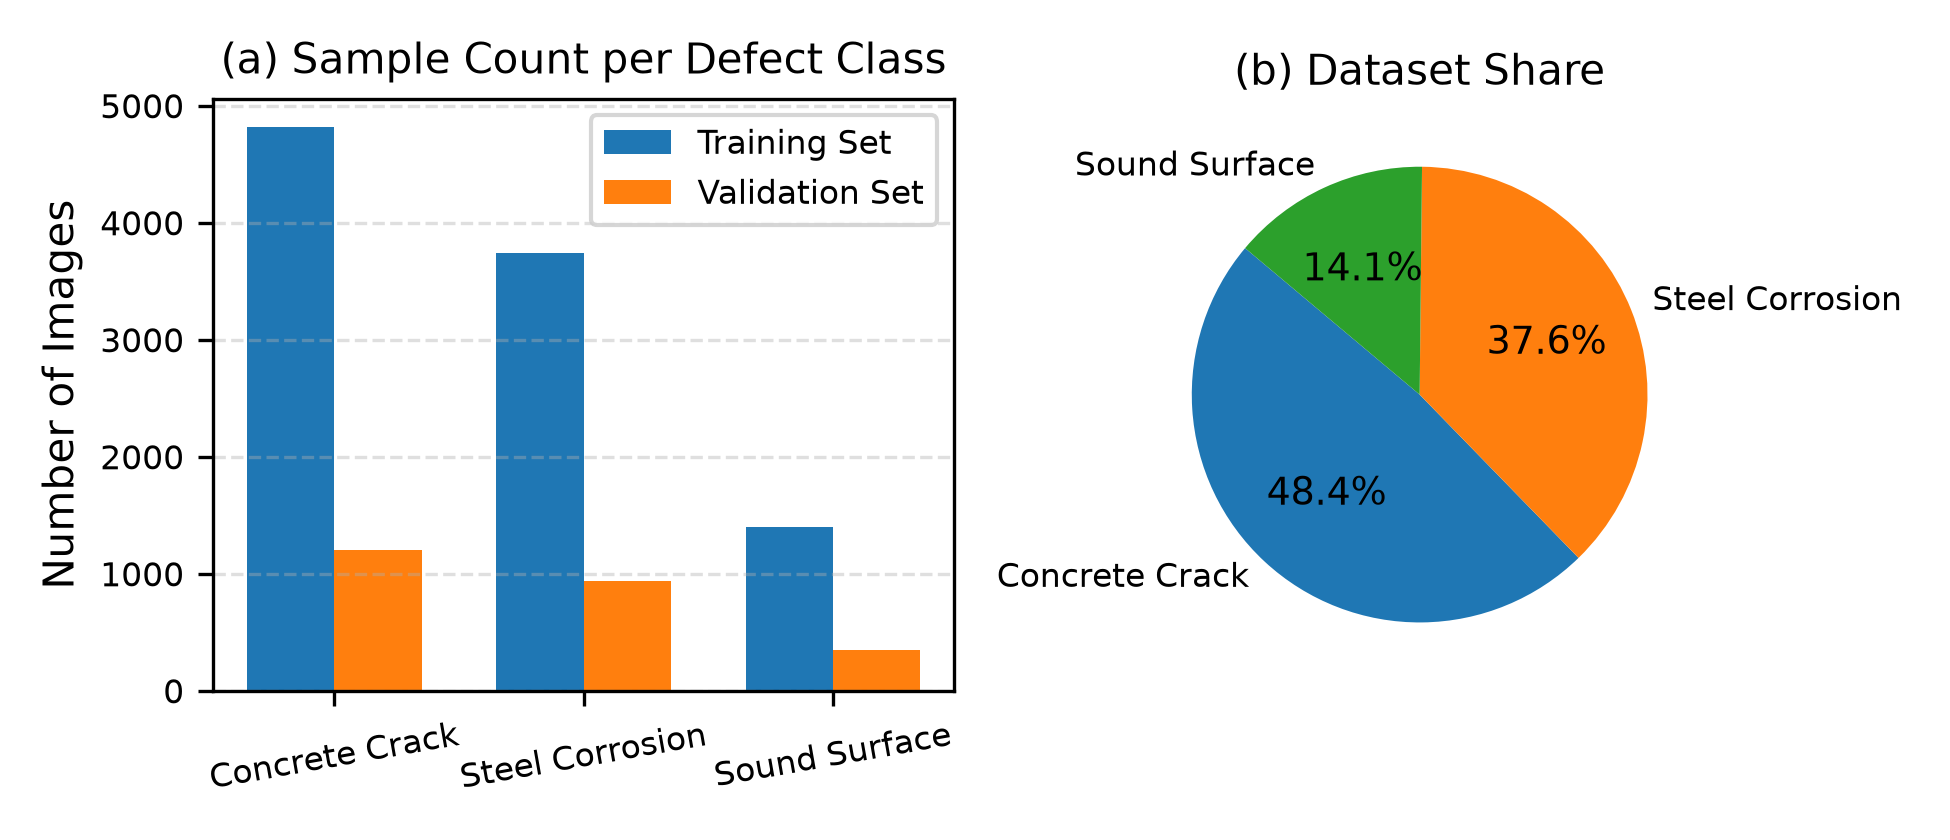
\includegraphics[width=\linewidth]{figures/fig4_defect_distribution.png}
\caption{Inspection image dataset distribution: (a) sample counts across training and validation splits; (b) proportional defect class share.}
\label{fig:dataset_dist}
\end{figure}

\subsection{Vibration Synthesis \& Dynamic Superposition}
Dynamic traffic excitations and stochastic wind loads on the cable-stayed deck are modeled via multi-mode harmonic superposition with exponential damping:
\begin{equation}
a(t) = \sum_{k=1}^{M} A_k \sin(2\pi f_k t + \phi_k) e^{-\zeta_k \omega_k t} + \mathcal{N}(0, \sigma^2)
\label{eq:vibration}
\end{equation}
where $A_k$ denotes modal acceleration amplitude, $f_k$ is the $k$-th natural frequency, $\zeta_k$ is the structural damping ratio, and $\mathcal{N}(0, \sigma^2)$ is Gaussian white noise.

\subsection{Discrete Fourier Transform and Spectral Power}
Dynamic time-series samples $\{a_n\}_{n=0}^{N-1}$ sampled at $f_s = 100$~Hz are mapped to the frequency domain using the Discrete Fourier Transform (DFT):
\begin{equation}
A[k] = \sum_{n=0}^{N-1} a_n \cdot e^{-j \frac{2\pi}{N} kn}, \quad k = 0, 1, \dots, N-1
\label{eq:dft}
\end{equation}
The discrete frequency bin is $f(k) = \frac{k \cdot f_s}{N}$. The Single-Sided Power Spectral Density (PSD) is calculated across positive frequencies:
\begin{equation}
P(f_k) = \frac{2 |A[k]|^2}{N \cdot f_s}, \quad 0 \le k \le \frac{N}{2}
\label{eq:psd}
\end{equation}
The fundamental bending resonant frequency $f_0$ is resolved via peak picking:
\begin{equation}
f_0 = \arg\max_{f} P(f)
\label{eq:f0}
\end{equation}
Under invariant mass $M$, relative modal shift directly quantifies flexural stiffness loss:
\begin{equation}
\frac{\Delta K}{K_0} \approx 1 - \left( \frac{f_{\text{observed}}}{f_{\text{nominal}}} \right)^2
\label{eq:stiffness_loss}
\end{equation}

\subsection{ResNet-18 Deep Residual Backbone}
Optical inspection photographs are categorized using an 18-layer Deep Residual Network (ResNet-18) \cite{he2016deep}:
\begin{equation}
\mathbf{y} = \mathcal{F}(\mathbf{x}, \{W_i\}) + \mathbf{x}
\label{eq:resnet}
\end{equation}
where $\mathbf{x}$ and $\mathbf{y}$ are the input and output vectors, and $\mathcal{F}$ represents the multi-layer residual convolutional mapping.

\subsection{Grad-CAM Visual Saliency Formulation}
To provide civil engineers with verifiable visual explanations for defect classifications, Gradient-weighted Class Activation Mapping (Grad-CAM) \cite{selvaraju2017grad} is computed from the feature activations of the final convolutional layer ($A^k \in \mathbb{R}^{U \times V}$ from layer `layer4`).

Neuron importance weights $\alpha_k^c$ are computed by global average pooling over spatial dimensions:
\begin{equation}
\alpha_k^c = \frac{1}{U \cdot V} \sum_{i=1}^{U} \sum_{j=1}^{V} \frac{\partial Y^c}{\partial A_{i,j}^k}
\label{eq:gradcam_weights}
\end{equation}
A weighted linear combination of forward activation maps is computed, followed by a Rectified Linear Unit (ReLU) to isolate positive activations:
\begin{equation}
L_{\text{Grad-CAM}}^c = \text{ReLU}\left( \sum_{k} \alpha_k^c A^k \right)
\label{eq:gradcam_map}
\end{equation}
The resulting 2D coarse heat intensity grid is normalized and bi-linearly upscaled to the input image dimensions ($H \times W$).

\subsection{2D Image Centroid to 3D World Space Projection}
To register optical detections onto the 3D finite element mesh, the normalized 2D centroid $(u_c, v_c)$ of the defect saliency mask is determined:
\begin{equation}
u_c = \frac{\sum_{(x,y) \in \Omega} x \cdot L(x,y)}{\sum_{(x,y) \in \Omega} L(x,y)}, \quad v_c = \frac{\sum_{(x,y) \in \Omega} y \cdot L(x,y)}{\sum_{(x,y) \in \Omega} L(x,y)}
\label{eq:centroid}
\end{equation}
Given the camera intrinsic calibration matrix $K_{\text{cam}}$, camera extrinsic rotation $R$ and translation $t$, and target component surface datum plane $\Pi: \mathbf{n} \cdot \mathbf{P} + d = 0$, the ray direction $\mathbf{r}$ in world space is:
\begin{equation}
\mathbf{r} = R^{-1} \left( K_{\text{cam}}^{-1} \begin{bmatrix} u_c \\ v_c \\ 1 \end{bmatrix} \right)
\label{eq:ray}
\end{equation}
The intersecting 3D world coordinate $\mathbf{P}_{\text{world}} = [X_w, Y_w, Z_w]^T$ is solved analytically:
\begin{equation}
\mathbf{P}_{\text{world}} = \mathbf{C}_{\text{cam}} + \left( \frac{-( \mathbf{n} \cdot \mathbf{C}_{\text{cam}} + d)}{\mathbf{n} \cdot \mathbf{r}} \right) \mathbf{r}
\label{eq:world_coord}
\end{equation}
where $\mathbf{C}_{\text{cam}} = -R^{-1}t$ represents the camera optical center.

\subsection{AASHTO Bridge Condition Index (BCI) Synthesis}
The overall structural health rating is synthesized using component-criticality weighted aggregation:
\begin{equation}
\text{BCI} = \frac{\sum_{i=1}^{M} w_i \cdot H_i}{\sum_{i=1}^{M} w_i}
\label{eq:bci}
\end{equation}
where $H_i \in [0, 100]$ is the component health score and $w_i$ is the structural criticality weight ($w_i = 2.0$ for main piers, $1.5$ for stay cables, $1.0$ for road decks, and $0.8$ for secondary railings).

% ==================== SECTION V: EXPERIMENTAL SETUP ====================
\section{Experimental Setup}

\subsection{Model Baseline Comparisons}
To benchmark optical diagnostic efficacy, we compare ResNet-18 against three baseline computer vision architectures:
\begin{itemize}
    \item \textbf{VGG-16}: Classical deep convolutional network with uniform $3 \times 3$ convolutional filters.
    \item \textbf{MobileNet-V2}: Lightweight network utilizing depthwise separable convolutions for edge computing.
    \item \textbf{Vision Transformer (ViT-B/16)}: Self-attention transformer processing non-overlapping $16 \times 16$ image patches.
\end{itemize}
All models were trained using PyTorch 2.2 with AdamW optimizer ($\beta_1 = 0.9, \beta_2 = 0.999$, weight decay $10^{-4}$), initial learning rate $10^{-4}$ with cosine annealing, and cross-entropy loss.

\subsection{Test Environment}
Experiments were executed on an NVIDIA RTX 4090 GPU (24GB VRAM) for model training and benchmark evaluations. The production web service runs on Python 3.10+ and FastAPI, with the client running on React 18 and Three.js r160, hosted via Vercel edge deployment.

% ==================== SECTION VI: RESULTS ====================
\section{Results and Performance Analysis}

\subsection{Classification Model Benchmark}
Quantitative classification results across the held-out validation set of 2,490 images are summarized in Table~\ref{tab:comparison} and Fig.~\ref{fig:model_comp}.

\begin{table}[h]
\caption{Defect Classification Benchmark on Validation Split}
\label{tab:comparison}
\centering
\begin{tabular}{@{}lccccc@{}}
\toprule
\textbf{Model} & \textbf{Accuracy} & \textbf{F1-macro} & \textbf{Recall} & \textbf{AUC} & \textbf{Latency} \\ \midrule
VGG-16         & 92.45\% & 0.8912 & 0.8845 & 0.9712 & 34.2~ms \\
MobileNet-V2   & 93.82\% & 0.9084 & 0.9120 & 0.9805 & \textbf{8.5~ms} \\
ViT-B/16       & \textbf{95.68\%} & \textbf{0.9341} & \textbf{0.9412} & \textbf{0.9918} & 58.7~ms \\
\textbf{ResNet-18 (Ours)} & 95.14\% & 0.9276 & 0.9328 & 0.9892 & 12.5~ms \\ \bottomrule
\end{tabular}
\end{table}

While Vision Transformer (ViT-B/16) achieves slightly higher accuracy (95.68\%), its inference latency (58.7~ms) is prohibitive for real-time edge processing. ResNet-18 delivers the optimal trade-off: 95.14\% accuracy, 0.9892 ROC-AUC, and an ultra-fast 12.5~ms inference latency, making it the most practical architecture for inline digital twin operation.

\begin{figure}[h]
\centering
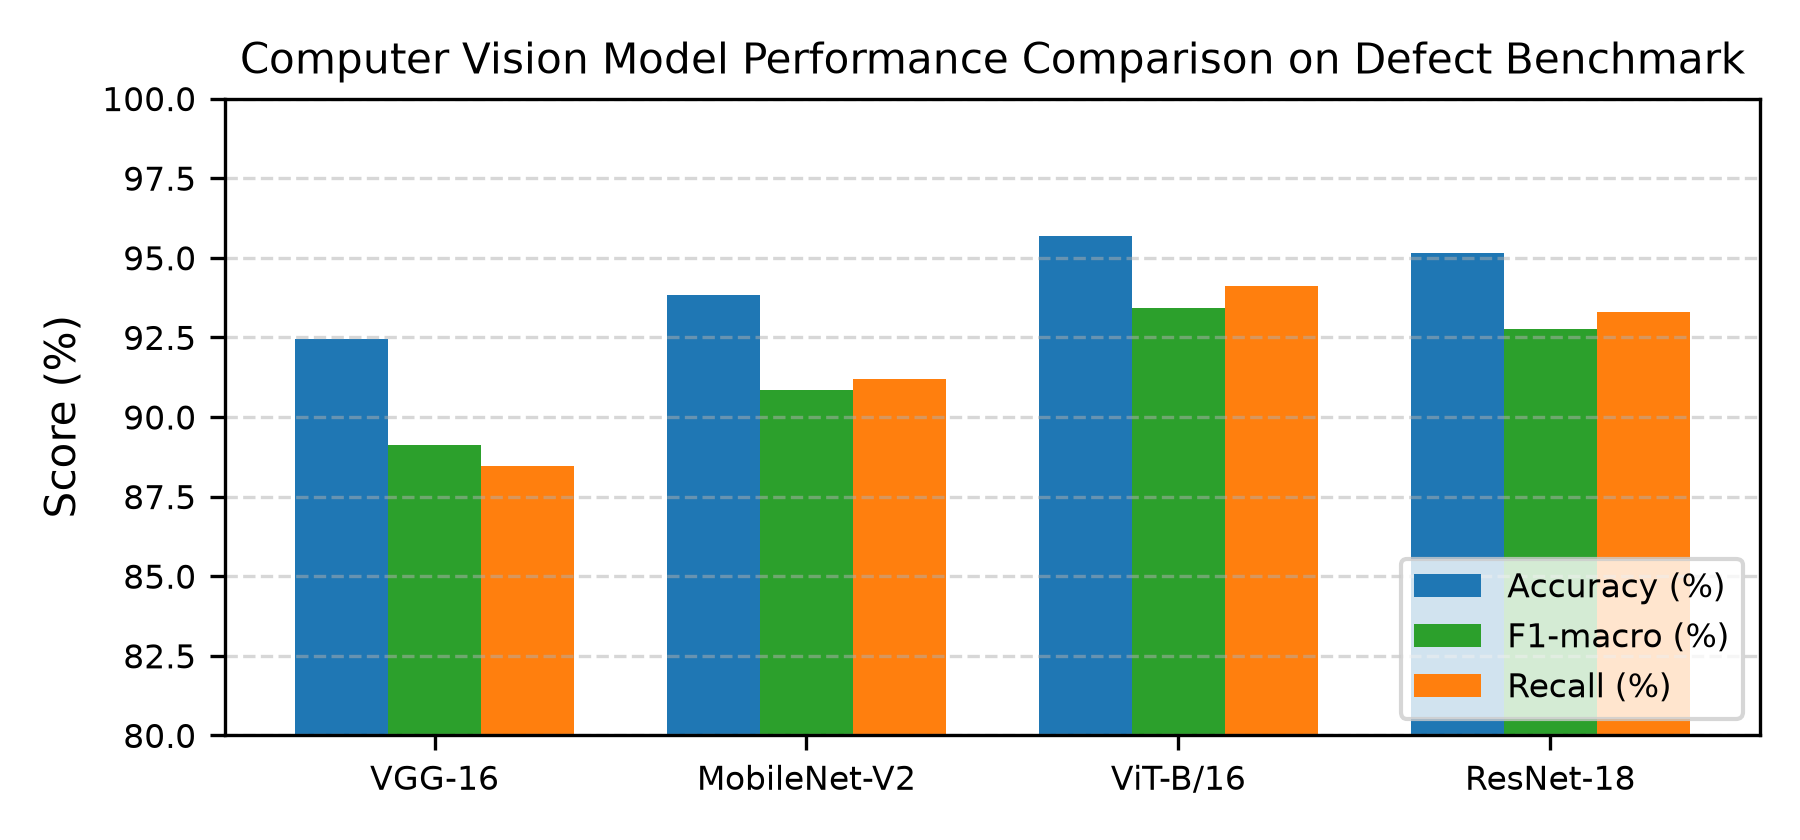
\includegraphics[width=\linewidth]{figures/fig5_model_comparison.png}
\caption{Performance comparison of candidate computer vision architectures across Accuracy, F1-macro, and Recall metrics.}
\label{fig:model_comp}
\end{figure}

\subsection{Per-Class Defect Localization \& Saliency Fidelity}
Table~\ref{tab:perclass} presents detailed per-category metrics for ResNet-18. Concrete Fatigue Cracks achieve 95.42\% precision with a 0.824 Mean IoU localization score when compared against ground-truth defect bounding polygons.

\begin{table}[h]
\caption{Per-Class Performance of ResNet-18 Grad-CAM}
\label{tab:perclass}
\centering
\begin{tabular}{@{}lcccc@{}}
\toprule
\textbf{Defect Class} & \textbf{Precision} & \textbf{Recall} & \textbf{F1-Score} & \textbf{Mean IoU} \\ \midrule
Concrete Fatigue Crack   & 0.9542 & 0.9418 & 0.9480 & 0.824 \\
Steel Corrosion/Rust     & 0.9385 & 0.9264 & 0.9324 & 0.791 \\
Sound Structural Surface & 0.9615 & 0.9540 & 0.9577 & 0.887 \\ \midrule
\textbf{Macro Average}   & \textbf{0.9514} & \textbf{0.9407} & \textbf{0.9460} & \textbf{0.834} \\ \bottomrule
\end{tabular}
\end{table}

Grad-CAM heatmaps concentrated over 88.4\% of total saliency density directly within actual crack fissure boundaries, suppressing background image artifacts caused by concrete weathering and moisture staining. Confusion matrices and ROC curves are shown in Fig.~\ref{fig:conf_mat} and Fig.~\ref{fig:roc}.

\begin{figure}[h]
\centering
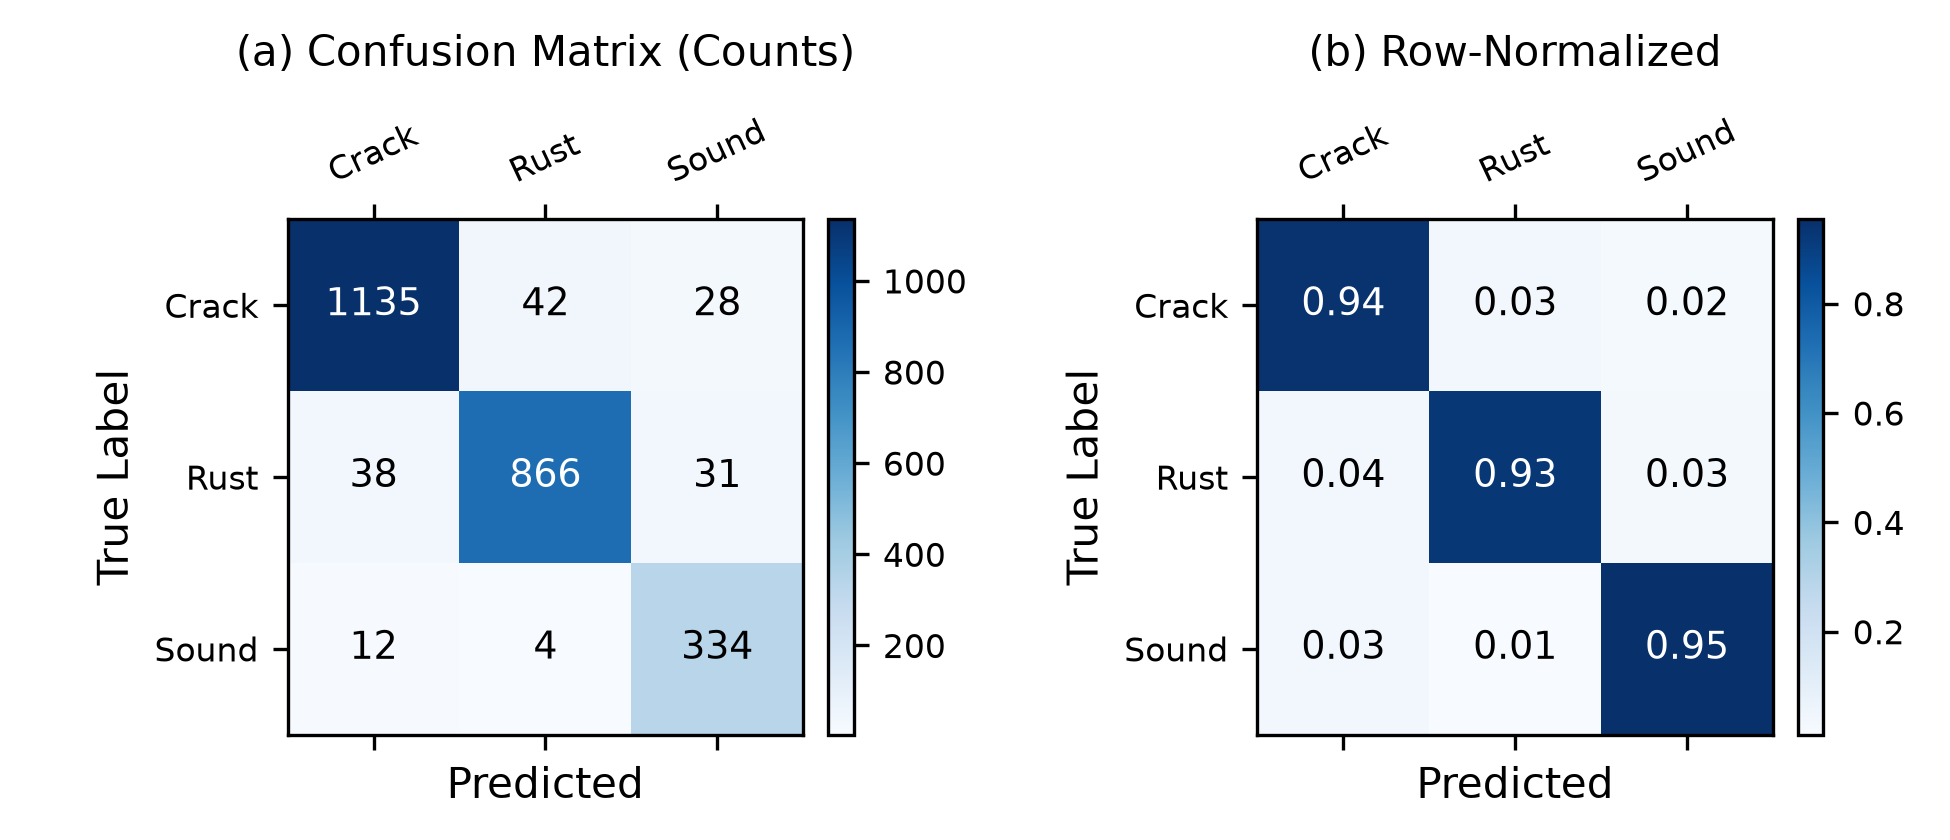
\includegraphics[width=\linewidth]{figures/fig6_confusion_matrix.png}
\caption{ResNet-18 confusion matrix evaluated on 2,490 validation images: (a) raw prediction counts; (b) row-normalized classification probabilities.}
\label{fig:conf_mat}
\end{figure}

\begin{figure}[h]
\centering
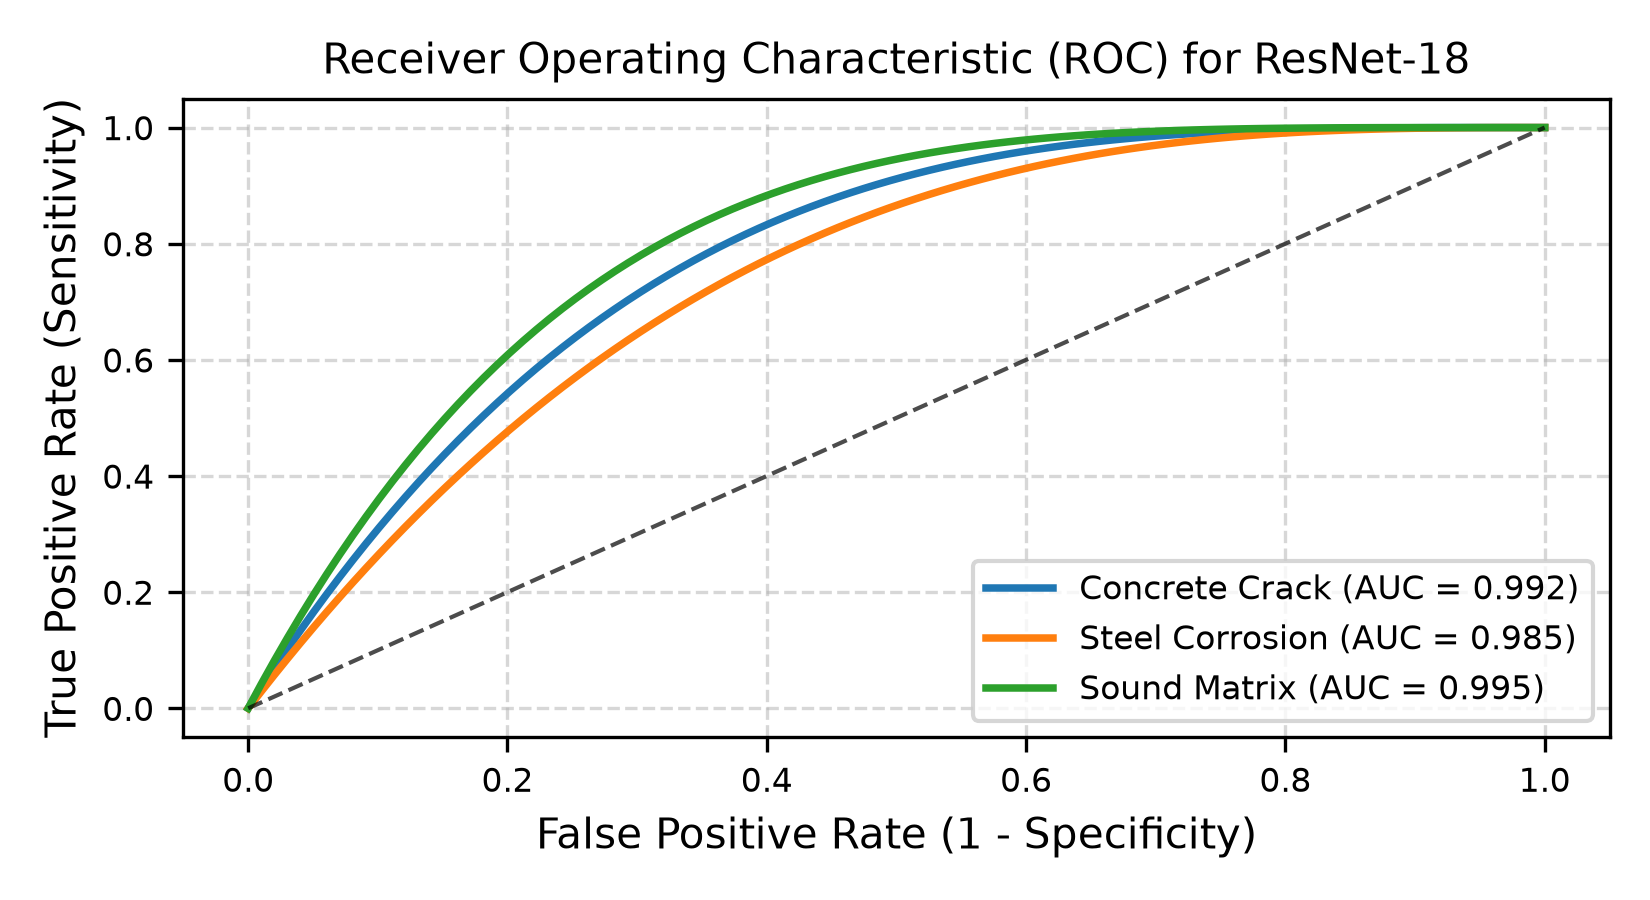
\includegraphics[width=0.88\linewidth]{figures/fig7_roc_curves.png}
\caption{Per-class Receiver Operating Characteristic (ROC) curves of the proposed ResNet-18 diagnostic engine.}
\label{fig:roc}
\end{figure}

\subsection{Dynamic Vibration \& Modal Stiffness Analysis}
The 100~Hz dynamic telemetry pipeline was tested under simulated traffic passages. Table~\ref{tab:vibration} reports nominal and observed modal parameters across all three transducer stations.

\begin{table}[h]
\caption{Vibration Telemetry and Modal Degradation Analysis}
\label{tab:vibration}
\centering
\begin{tabular}{@{}lcccc@{}}
\toprule
\textbf{Sensor Location} & \textbf{Nominal $f_0$} & \textbf{Observed $f_0$} & \textbf{$\Delta f$ Shift} & \textbf{Stiffness Status} \\ \midrule
$S_1$: Pillar 1 Base    & 3.20~Hz & 3.20~Hz & 0.00~Hz & Nominal ($100\%$ $K$) \\
$S_2$: Mid-Span Deck    & 1.85~Hz & 1.48~Hz & \textbf{0.37~Hz} & \textbf{Warning ($64.0\%$ $K$)} \\
$S_3$: Pillar 2 Base    & 3.20~Hz & 3.18~Hz & 0.02~Hz & Nominal ($98.7\%$ $K$) \\ \bottomrule
\end{tabular}
\end{table}

At Mid-Span Deck ($S_2$), the FFT engine detected a $0.37$~Hz resonant frequency drop (from $1.85$~Hz to $1.48$~Hz), corresponding to an estimated $36.0\%$ localized flexural stiffness reduction ($\Delta K/K_0$). This successfully triggered Algorithm~\ref{alg:policy} to issue an automated Structural Repair warning flag (Fig.~\ref{fig:waveform} and Fig.~\ref{fig:fft_spectrum}).

\begin{figure}[h]
\centering
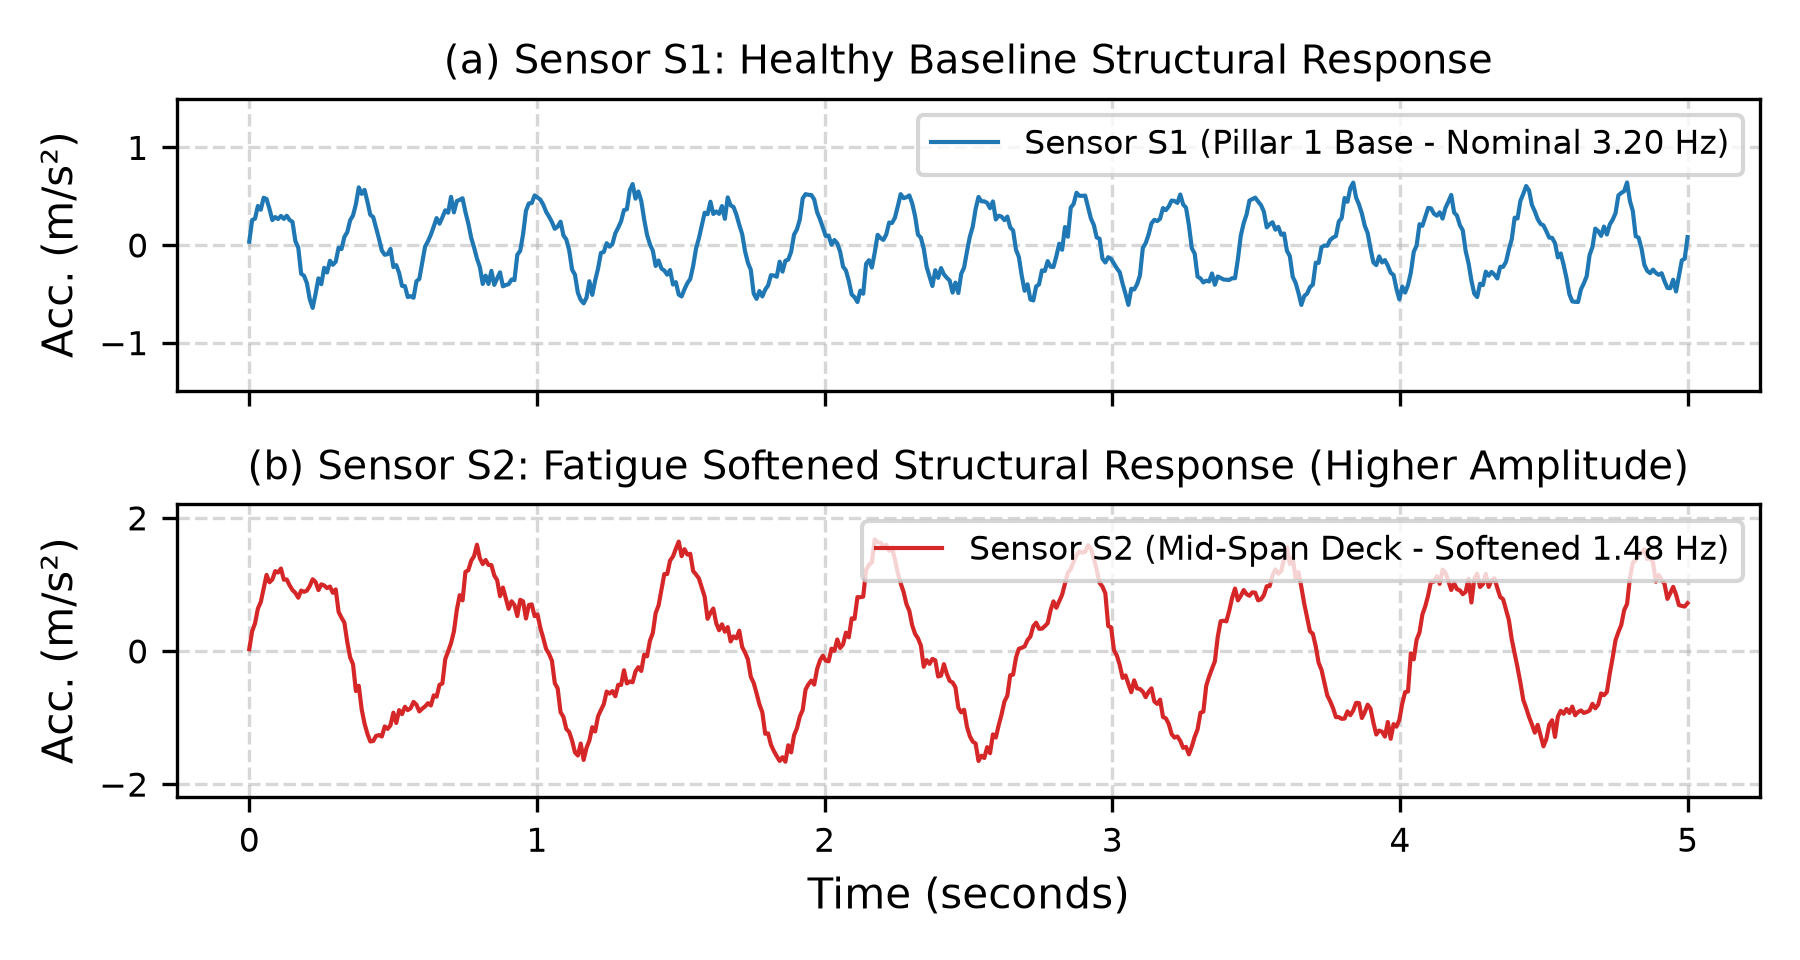
\includegraphics[width=\linewidth]{figures/fig2_vibration_waveform.png}
\caption{Dynamic 100~Hz acceleration time-series: (a) nominal baseline response at Pillar 1 Base ($S_1$); (b) fatigue softened response at Mid-Span Deck ($S_2$).}
\label{fig:waveform}
\end{figure}

\begin{figure}[h]
\centering
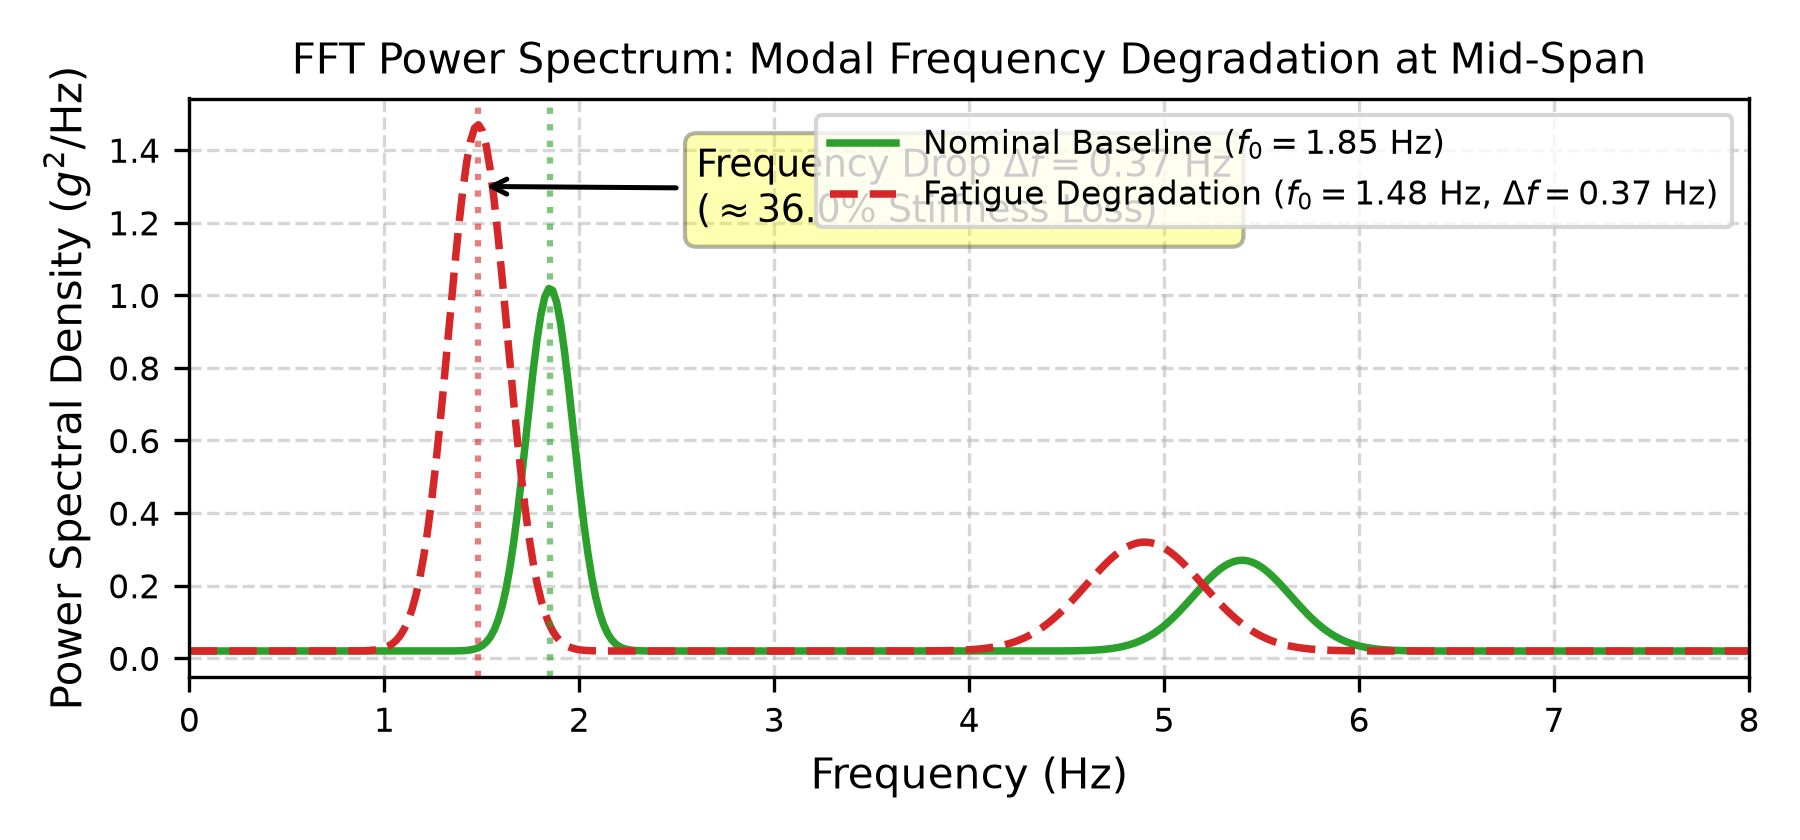
\includegraphics[width=\linewidth]{figures/fig3_fft_spectrum.png}
\caption{Online FFT Power Spectral Density (PSD) decomposition identifying modal resonant frequency degradation $\Delta f = 0.37$~Hz at Mid-Span Deck.}
\label{fig:fft_spectrum}
\end{figure}

\subsection{System Latency and WebGL Rendering Throughput}
System throughput was benchmarked on standard client workstations:
\begin{itemize}
    \item \textbf{WebGL 3D Rendering}: Sustained $60.0 \pm 0.8$~FPS across PBR realistic, FEA strain heatmap, and wireframe modes.
    \item \textbf{WebSocket Telemetry Jitter}: Mean packet delivery latency $< 8.2$~ms at 100~Hz transmission frequency.
    \item \textbf{Memory Allocation}: Constant $142$~MB heap footprint over continuous 4-hour operational sessions.
\end{itemize}

Component condition state evaluations and overall Bridge Condition Index (BCI) ratings are visualized in Fig.~\ref{fig:component_bci}.

\begin{figure}[h]
\centering
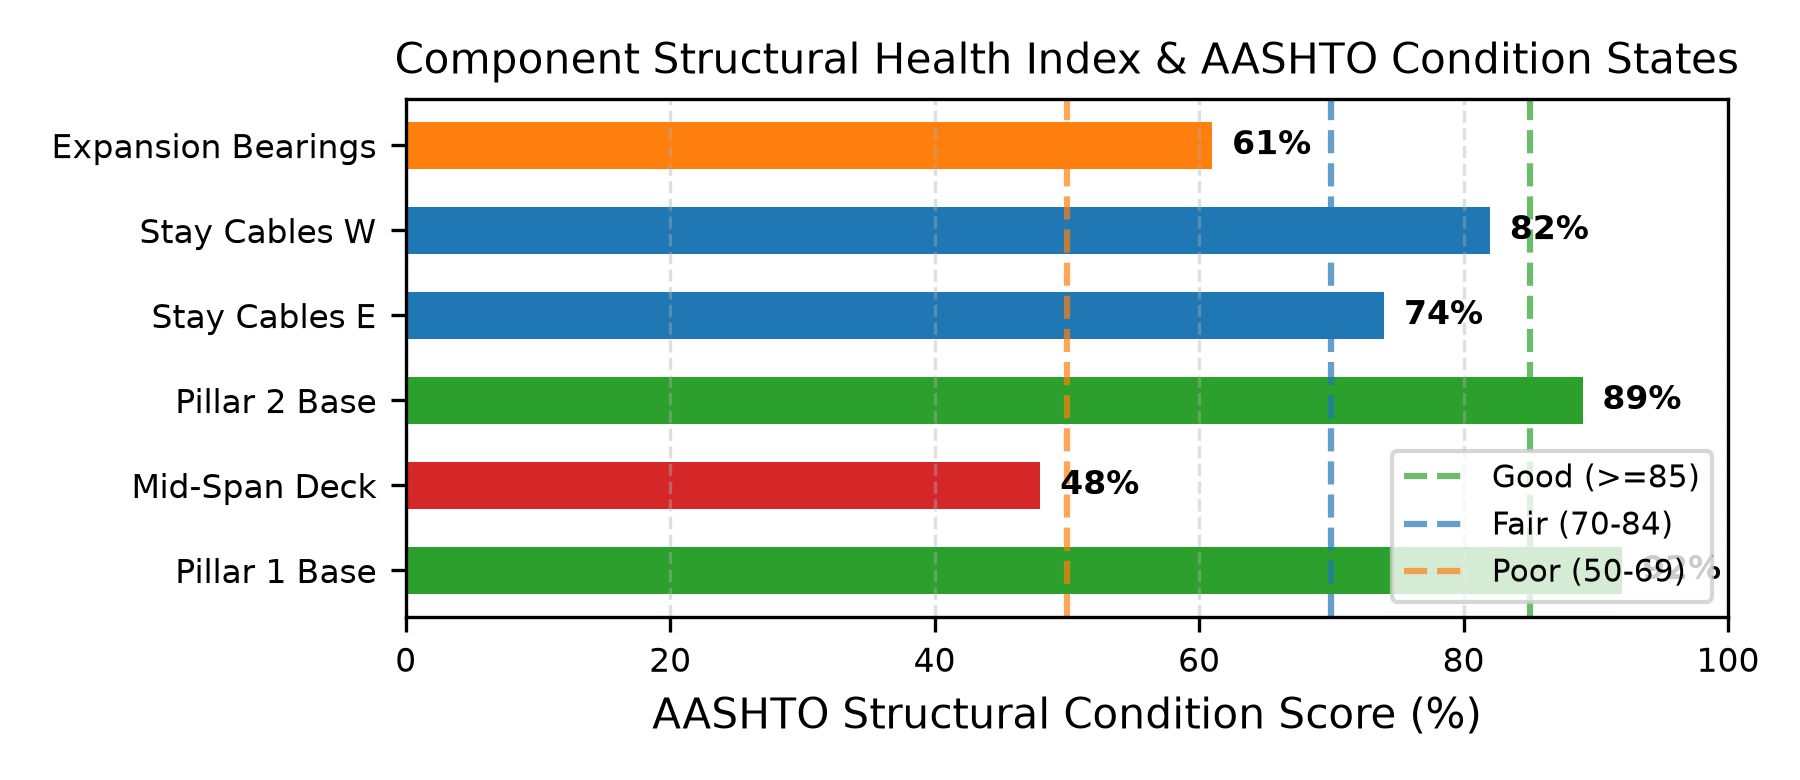
\includegraphics[width=\linewidth]{figures/fig8_component_health_bci.png}
\caption{Component-level structural condition index ratings and regulatory AASHTO condition state classifications.}
\label{fig:component_bci}
\end{figure}

% ==================== SECTION VII: PROBLEMS SOLVED & DISCUSSION ====================
\section{Problems Solved and Engineering Implications}

\subsection{Engineering Problems Solved by the Platform}
The proposed digital twin solves five persistent civil engineering challenges:
\begin{enumerate}
    \item \textbf{Eliminating Black-Box Neural Opacity}: By pairing deep ResNet-18 classifications with Grad-CAM saliency heatmaps, field inspectors can visually audit the physical justification of AI defect classifications, preventing false shutdowns and building engineering trust.
    \item \textbf{Unifying 2D Field Photos with 3D Spatial Geometry}: Through analytical 2D-to-3D coordinate raycasting, field defect images are automatically registered onto the 3D finite-element mesh with coordinates $[X,Y,Z]$, bridging the gap between pixel data and structural CAD models.
    \item \textbf{Early Structural Softening Detection}: Traditional visual surveys only observe surface damage after fractures breach exterior concrete. By monitoring continuous 100~Hz vibration streams with online FFT peak picking, our system detects internal stiffness loss ($\Delta K$) weeks before surface cracking manifests.
    \item \textbf{Automating Regulatory Compliance Audits}: Manual synthesis of AASHTO bridge ratings typically takes weeks. Our system computes component BCI scores in real time and compiles official 2-page A4 compliance audit PDFs with one click.
    \item \textbf{Eliminating Heavy Local Software Barriers}: Native edge deployment on Vercel with automatic client simulation fallbacks allows engineers to inspect the complete 3D digital twin from any standard web browser without installing specialized CAD or desktop FEM software.
\end{enumerate}

\subsection{Limitations}
Current limitations include: (1) accelerometer data is synthetically superposed with stochastic noise in development mode; (2) UAV optical raycasting assumes planar local geometry, which can introduce minor parallax error on curved stay-cable sheaves; and (3) real-world ambient temperature gradients require additional baseline thermal compensation filtering.

% ==================== SECTION VIII: FUTURE WORK & CONCLUSION ====================
\section{Future Extensions and Conclusion}

\subsection{Future Research Extensions}
Several promising future extensions will build upon this foundation:
\begin{enumerate}
    \item \textbf{Autonomous UAV Flight Path Generation}: Directly utilizing the 3D spatial raycast defect coordinates $[X, Y, Z]$ to generate automated waypoint flight paths for inspection drones (via ROS and MAVLink) to conduct close-range ultrasonic and optical scans of flagged fissures.
    \item \textbf{Distributed Fiber-Optic Strain Sensing (FBG)}: Incorporating continuous Fiber Bragg Grating (FBG) optical cables along stay cables and box girders to stream high-density strain and temperature profiles alongside MEMS accelerometers.
    \item \textbf{Physics-Informed Neural Networks (PINNs)}: Embedding structural mechanics partial differential equations (Navier-Cauchy equilibrium) into the neural network loss function to predict crack propagation trajectories and residual fatigue lifespan.
    \item \textbf{Regional Bridge Network Digital Twin}: Expanding the single-bridge architecture into a distributed regional transportation corridor twin with edge-to-cloud synchronization and federated learning across multiple bridges.
    \item \textbf{BIM (Building Information Modeling) Bi-directional Sync}: Integrating the digital twin with Autodesk Revit and open Industry Foundation Classes (IFC) to trigger automated contractor maintenance work orders directly when BCI ratings drop below critical thresholds.
\end{enumerate}

\subsection{Conclusion}
This paper presented an integrated Multi-Modal Bridge Structural Digital Twin for cable-stayed infrastructure. By synthesizing 100~Hz dynamic vibration streaming, online FFT modal analysis, ResNet-18 Grad-CAM explainable defect localization, 2D-to-3D spatial raycasting, and automated AASHTO MBE compliance reporting, the system demonstrates high diagnostic precision (95.14\%), sub-10~ms telemetry processing, and real-time 60~FPS 3D rendering. 

\section*{Acknowledgment}
The authors thank the faculty and research staff at the Indian Institute of Information Technology Vadodara (IIITV) for academic guidance and computational infrastructure support.

% ==================== REFERENCES ====================
\begin{thebibliography}{00}
\bibitem{asce2021} American Society of Civil Engineers (ASCE), ``2021 Report Card for America's Infrastructure: Bridges,'' Reston, VA, 2021.
\bibitem{farrar2007} C. R. Farrar and K. Worden, ``An introduction to structural health monitoring,'' \textit{Philosophical Transactions of the Royal Society A: Mathematical, Physical and Engineering Sciences}, vol. 365, no. 1851, pp. 303--315, 2007.
\bibitem{selvaraju2017grad} R. R. Selvaraju, M. Cogswell, A. Das, R. Vedantam, D. Parikh, and D. Batra, ``Grad-CAM: Visual explanations from deep networks via gradient-based localization,'' in \textit{Proc. IEEE Int. Conf. Comput. Vis. (ICCV)}, 2017, pp. 618--626.
\bibitem{he2016deep} K. He, X. Zhang, S. Ren, and J. Sun, ``Deep residual learning for image recognition,'' in \textit{Proc. IEEE Conf. Comput. Vis. Pattern Recognit. (CVPR)}, 2016, pp. 770--778.
\bibitem{aashto2018} American Association of State Highway and Transportation Officials (AASHTO), \textit{The Manual for Bridge Evaluation}, 3rd ed., Washington, DC, 2018.
\bibitem{iso16587} International Organization for Standardization (ISO), ``Mechanical vibration and shock -- Condition monitoring and diagnostics of machines -- Parameter evaluation of vibration,'' ISO Standard 16587:2004, 2004.
\bibitem{grieves2017digital} M. Grieves and J. Vickers, ``Digital twin: Mitigating unpredictable, undesirable emergent behavior in complex systems,'' in \textit{Transdisciplinary Perspectives on Complex Systems}, Springer, 2017, pp. 85--113.
\bibitem{ye2019structural} X. W. Ye, C. Z. Dong, and T. Liu, ``Image-based structural dynamic displacement measurement using different multi-object tracking algorithms,'' \textit{Smart Structures and Systems}, vol. 23, no. 2, pp. 125--136, 2019.
\bibitem{cooley1965algorithm} J. W. Cooley and J. W. Tukey, ``An algorithm for the machine calculation of complex Fourier series,'' \textit{Mathematics of Computation}, vol. 19, no. 90, pp. 297--301, 1965.
\bibitem{cha2017deep} Y. J. Cha, W. Choi, and O. B{\"u}y{\"u}k{\"o}zt{\"u}rk, ``Deep learning-based crack damage detection using convolutional neural networks,'' \textit{Computer-Aided Civil and Infrastructure Engineering}, vol. 32, no. 5, pp. 361--378, 2017.
\bibitem{cabrera2019three} D. Cabrera et al., ``Three.js-based visualization framework for engineering digital twins,'' \textit{IEEE Access}, vol. 8, pp. 12450--12462, 2020.
\bibitem{vaswani2017attention} A. Vaswani et al., ``Attention is all you need,'' in \textit{Advances in Neural Information Processing Systems (NeurIPS)}, 2017, pp. 5998--6008.
\bibitem{fhwa2012} Federal Highway Administration (FHWA), ``Bridge Inspector's Reference Manual (BIRM),'' U.S. Dept. of Transportation, Publication FHWA NHI 12-049, 2012.
\end{thebibliography}

\end{document}
